\documentclass[12pt]{iopjournal}

\usepackage{bm}
\usepackage{amssymb}
\usepackage{booktabs}
\usepackage{mathtools}
\usepackage{microtype}
\usepackage{amsthm}
\usepackage{url}
\usepackage{placeins}
\usepackage[backend=biber,style=numeric-comp,sorting=none,giveninits=true,maxbibnames=99]{biblatex}
\addbibresource{references.bib}

\hypersetup{
  colorlinks=true,
  allcolors=blue,
  pdftitle={Detector-Restricted Identifiability of Charged Spin-1/2 and Spin-1 Particles: Whole-Class Certificates and Exact Degeneracies},
  pdfauthor={Dino Vlahek},
  pdfkeywords={charged-particle spin, identifiability, detector bandwidth, electromagnetic form factors, inverse problems, quantum field theory}
}

\newcommand{\Hs}{\mathcal H_s}
\newcommand{\Mcal}{\mathfrak M}
\newcommand{\Dcal}{\mathcal D}
\newcommand{\Pcal}{\mathcal P}
\newcommand{\Tcal}{\mathcal T}
\newcommand{\Wbar}{\overline{\bm W}}
\newcommand{\dd}{\mathrm d}
\newcommand{\DKL}{D_{\mathrm{KL}}}
\newcommand{\Tr}{\operatorname{Tr}}
\newcommand{\diag}{\operatorname{diag}}
\newcommand{\rank}{\operatorname{rank}}
\providecommand{\alttext}[1]{}

\newtheorem{theorem}{Theorem}[section]
\newtheorem{lemma}{Lemma}[section]
\newtheorem{proposition}{Proposition}[section]
\newtheorem{corollary}{Corollary}[section]
\theoremstyle{definition}
\newtheorem{definition}{Definition}[section]
\theoremstyle{remark}
\newtheorem{remark}{Remark}[section]

\setlength{\headheight}{15pt}
% Author-prepared review PDF: replace template-only production headers.
\renewcommand{\articletype}[1]{\par\noindent\textsf{\textbf{#1}}\par\medskip}
\AtBeginDocument{%
  \fancyhfoffset[L]{0pt}
  \fancyhead[L]{\small Detector-restricted spin identifiability}
  \fancyhead[R]{\small D. Vlahek}
  \renewcommand{\headrulewidth}{0.3pt}
}

\begin{document}

\articletype{Paper}

\title{Detector-Restricted Identifiability of Charged Spin-$1/2$ and Spin-$1$ Particles: Whole-Class Certificates and Exact Degeneracies}

\author{Dino Vlahek}\par
\affil{Laboratory for Data Mining and Intelligent Systems, Faculty of Organization and Informatics, University of Zagreb, Pavlinska 2, 42000 Vara\v{z}din, Croatia}
\par\email{dvlahek@foi.hr}\par
\par\keywords{charged-particle spin, identifiability, detector bandwidth, electromagnetic form factors, inverse problems, quantum field theory}

\begin{abstract}
A particle's spin is intrinsic, but identifying it requires responses that a detector can access. We study charged spin-$1/2$ and spin-$1$ candidates through calibrated magnetic and charge-sensitive rank-$2$ responses. The absence of an internal rank-$2$ sector for spin $1/2$ and Haberzettl's elementary-field moment relation define a reference current class. We determine the primitive detector resources needed to distinguish the two classes with uncertain electromagnetic form factors and test robustness under the deformation $g_M+g_Q=1+\delta$. For $g_M\in[1,3]$, the magnetic channel alone separates the full anchored Lipschitz class at every finite Gaussian bandwidth and finite Lipschitz bound, independently of $\delta$. On the $\delta=0$ slice, the broader class $g_M\in[-4,4]$ contains $63$ whole-class certified points, $33$ exact overlaps, and three unresolved points on a $99$-point bandwidth--smoothness grid. A uniform $|\delta|\le0.10$ enlargement retains $61$ whole-class certificates, while all existing overlap witnesses remain admissible. The result makes the dependence of spin identifiability on detector architecture and the admitted nuisance class explicit at finite resolution.
\end{abstract}

% ============================================================
\section{Introduction}
\label{sec:introduction}

A detector does not read out a particle's spin directly. It records currents, decay products, polarization-dependent rates, and reconstructed momenta. Spin itself is a representation label of the Poincar\'e group \cite{Wigner1939}. The problem is to determine which information about that label survives the available interactions and detector responses.

Two different spin classes can give the same measured response when the detector is blind to their distinguishing component. More data then reproduce the same distribution more precisely. A different physical response, or an independently justified restriction on the candidate models, is needed to separate the classes.

Several established frameworks touch different parts of this question. Restricted-measurement distinguishability asks how well quantum states can be separated when only a limited measurement family is available \cite{MatthewsWehnerWinter2009}. Informational completeness studies which measurement sets determine states within specified classes \cite{Finkelstein2004,FlammiaSilberfarbCaves2005,BaldwinDeutschKalev2016}. Complete-experiment analyses seek minimal sets of observables sufficient to reconstruct reaction amplitudes \cite{ArenhoevelFix2014,TiatorWorkmanWunderlichHaberzettl2017,KroenertWunderlichAfzalThiel2021}. Quantum-system identification and observability address recovery of dynamical models from input-output records \cite{BurgarthYuasa2012,BurgarthYuasa2014,LeghtasTuriniciRabitzRouchon2012}. Operational equivalence and measurement-resource limitations also appear in recent work on quantum reference frames and restricted channels \cite{CaretteGlowackiLoveridge2023,SiddiquiWang2026,DuEtAl2026}. We focus on the elementary-particle spin label within a specified current and detector-response class.

The Quantum Temporal Probabilities (QTP) framework makes the detector dependence explicit. Measured probabilities are contractions of QFT correlation functions with a kernel containing the detector state, spectrum, coupling, and pointer coarse graining \cite{AnastopoulosSavvidou2015I,AnastopoulosSavvidou2015II,AnastopoulosSavvidou2022}. Recent work has applied this construction to relativistic spin and polarization measurements \cite{KoliopoulouAnastopoulosSavvidou2026}. We use this structure to motivate the detector-relative response map and positivity of the calibrated response blocks. The identifiability results require the positive measures specified below and do not depend on a complete process-specific QTP realization. We ask the inverse question and determine which representations remain compatible with a measured response.

Our example compares charged spin-$1/2$ and spin-$1$ particles. Electromagnetic multipole decompositions are established \cite{Lorce2009Part1,Lorce2009NaturalMoments,CotognoLorceLowdonMorales2020,CosynVera2025,HuangTanWangYu2026}. Spin $1/2$ has no internal rank-$2$ sector, and Haberzettl's elementary-field current relation constrains the magnetic and quadrupole moments of spin $1$ \cite{Haberzettl2019}. These facts alone do not determine which detector response separates the two classes once finite bandwidth and uncertain form factors are included. We formulate that question as separation of complete detector-response model sets.

We derive the minimum support in primitive magnetic and charge-sensitive responses and calculate finite-width bounds over the complete anchored Lipschitz class. Under a compact prior near the tree-level value $g_M=2$ \cite{FerraraPorratiTelegdi1992,BrodskyHiller1992,HagiwaraPecceiZeppenfeldHikasa1987}, the magnetic channel alone separates the classes for every finite bandwidth and Lipschitz bound. Enlarging the class to include its blind point changes the result. We then construct exact overlaps and certify the region in which the two-channel response remains separated. We also relax the exact moment relation by writing $g_M+g_Q=1+\delta$ and derive bounds uniform over $|\delta|\le\Delta$.

We use a calibrated positive two-channel model for elastic current matrix elements. Mapping these responses to observables is process dependent for a specific particle. For unstable vectors, polarization and spin information can be reconstructed from production and decay distributions \cite{BurnsKongMatchevPark2008,GaoEtAl2010,BolognesiEtAl2012,ChoiChristensenSalmonWang2015}. The present analysis concerns the information carried by the calibrated electromagnetic response blocks once such observables are available.

\section{Detector-relative representation identifiability}
\label{sec:operational}
% ============================================================

Let $\Mcal$ be a specified class of candidate QFT models and let $\Dcal=\{D_\alpha\}$ be a family of physical measurement channels. For $M\in\Mcal$ and $D_\alpha\in\Dcal$, let $P_{M,\alpha}$ be the probability law on the outcome space $\mathcal X_\alpha$. The detector-response map is
\begin{equation}
\Phi_{\Dcal}:\Mcal\rightarrow
\prod_{D_\alpha\in\Dcal}\Pcal(\mathcal X_\alpha),
\qquad
M\mapsto\{P_{M,\alpha}\}_{D_\alpha\in\Dcal},
\label{eq:response-map}
\end{equation}
where $\Pcal(\mathcal X_\alpha)$ is the set of probability measures on $\mathcal X_\alpha$.

\begin{definition}
\textbf{Detector-relative equivalence.}
Two models $M_1,M_2\in\Mcal$ are equivalent under $\Dcal$, written $M_1\sim_{\Dcal}M_2$, if
\begin{equation}
P_{M_1,\alpha}=P_{M_2,\alpha}
\qquad\text{for every }D_\alpha\in\Dcal.
\end{equation}
\end{definition}

The corresponding operational quotient is
\begin{equation}
\Mcal_{\mathrm{op}}(\Dcal)=\Mcal/\!\sim_{\Dcal}.
\end{equation}
Let $L:\Mcal\rightarrow\Lambda$ denote a structural label, such as the fundamental spin representation.

\begin{definition}
\textbf{Detector-relative label identifiability.}
The label $L$ is identifiable under $\Dcal$ if
\begin{equation}
M_1\sim_{\Dcal}M_2
\quad\Longrightarrow\quad
L(M_1)=L(M_2).
\end{equation}
\end{definition}

\paragraph{Infinite-statistics consequence.}
If $M_1\sim_{\Dcal}M_2$, no decision rule based only on repeated uses of channels in $\Dcal$ can consistently distinguish them. Every allowed single-trial distribution is identical under the two models, and therefore so is every joint distribution generated by independent repetition. If $P_{M_i}^{(n)}$ denotes the joint law for any fixed $n$-trial protocol, then
\begin{equation}
\DKL(P_{M_1}^{(n)}\Vert P_{M_2}^{(n)})=0,
\qquad
\|P_{M_1}^{(n)}-P_{M_2}^{(n)}\|_{\mathrm{TV}}=0.
\end{equation}
For equal priors, the optimal binary Bayes error remains $1/2$ for every $n$.

To count physical resources, the response coordinates must retain their detector architecture. Let $\mathcal A$ index primitive response blocks and write
\begin{equation}
\mathcal R_{\mathcal A}=\bigoplus_{a\in\mathcal A}\mathcal R_a.
\label{eq:block-architecture}
\end{equation}
For a label $\lambda$, let $\mathcal W_\lambda\subset\mathcal R_{\mathcal A}$ be the response model set generated by its admitted nuisance class, and let $\pi_S$ project onto the blocks in $S\subseteq\mathcal A$. We define the architecture-aware threshold
\begin{equation}
\boxed{
\tau_{\mathcal A}(\lambda,\lambda')=
\min_{S\subseteq\mathcal A}
\left\{|S|:\pi_S\mathcal W_\lambda
\cap\pi_S\mathcal W_{\lambda'}=\varnothing\right\}.}
\label{eq:general-threshold}
\end{equation}
The value is infinite if no allowed finite block subset separates the classes. It counts distinct primitive response types. Repeated samples and post-processed output dimension do not change this count.

\paragraph{Architecture invariance.}
The threshold in Eq.~\eqref{eq:general-threshold} is invariant under invertible changes of basis within each block $\mathcal R_a$, relabeling of the blocks, and invertible post-processing of the outputs from any fixed subset $S$. Each allowed transformation maps $\pi_S\mathcal W_\lambda$ and $\pi_S\mathcal W_{\lambda'}$ bijectively into transformed sets and preserves emptiness of their intersection and the value of $|S|$. Mixing different physical blocks is different because the mixed coordinate already requires joint access to those blocks.

For a linear scalar readout $L:\mathcal R_{\mathcal A}\to\mathbb R$, its architecture support is
\begin{align}
\operatorname{supp}_{\mathcal A}(L)
&=\{a\in\mathcal A:L|_{\mathcal R_a}\ne0\},
\notag\\
c_{\mathcal A}(L)
&=|\operatorname{supp}_{\mathcal A}(L)|.
\label{eq:readout-support}
\end{align}
Thus one scalar output can still use several physical resources. This distinction becomes explicit in the magnetic--charge example below.

% ============================================================
\section{QFT detector response and spin tensors}
\label{sec:qtp}
% ============================================================

\subsection{QTP detector kernel}

Consider a local interaction
\begin{equation}
\hat H_I(x)=\hat C_a(x)\otimes\hat J^a(x),
\end{equation}
where $\hat C_a$ is a local field operator and $\hat J^a$ is an apparatus current. To leading order, QTP assigns an unnormalized event probability density of the form \cite{AnastopoulosSavvidou2015I,AnastopoulosSavvidou2015II,AnastopoulosSavvidou2022,KoliopoulouAnastopoulosSavvidou2026}
\begin{equation}
P(x,\lambda)=\int\dd^4y\,R^{ab}(y,\lambda)
G_{ab}\!\left(x-\frac y2,x+\frac y2\right),
\label{eq:qtp-probability}
\end{equation}
where
\begin{equation}
G_{ab}(x,x')=\langle\psi|\hat C_a(x)\hat C_b(x')|\psi\rangle
\end{equation}
and
\begin{equation}
R^{ab}(y,\lambda)=
\langle\Omega|\hat J^a(x_0)\hat\Pi(\lambda)
 e^{-i\hat P\cdot y}\hat J^b(x_0)|\Omega\rangle.
\label{eq:detector-kernel}
\end{equation}
The detector state, spectrum, coupling, and pointer coarse graining are therefore part of the probability assignment.

When absorbed momentum is resolved, the spectral kernel has the positive form
\begin{equation}
\widetilde R^{ab}(k,Q)=2\pi
\langle\Omega|\hat J^a(x_0)\delta^4(\hat P-k)
\hat J^b(x_0)|\Omega\rangle\chi(k-Q).
\label{eq:spectral-kernel}
\end{equation}
For each $k$, $\widetilde R^{ab}$ is positive semidefinite in the current indices.
For a fixed pointer bin, the nonnegative window $\chi(k-Q)$ can be absorbed into a baseline spectral weight. We choose a centered Gaussian detector window below, with no additional transfer-dependent charge-sector filter. The resulting charge weight follows from the squared longitudinal current.

\subsection{One-particle response and irreducible transfer}

Let the measured state lie in a massive one-particle sector $\mathcal H_{m,s}$ with internal spin space $\Hs\simeq\mathbb C^{2s+1}$. Define one-particle current matrix elements
\begin{equation}
\Gamma^{a,(s)}_{\alpha r}(q,p)=\langle q,\alpha|\hat C^a(0)|p,r\rangle.
\end{equation}
The elastic one-particle response tensor is
\begin{equation}
B^{ab,(s)}_{rr'}(q,p,p')=
\sum_{\alpha=-s}^{s}
\Gamma^{a,(s)*}_{\alpha r}(q,p)
\Gamma^{b,(s)}_{\alpha r'}(q,p'),
\label{eq:response-tensor}
\end{equation}
and the detector-induced effect on the internal space is, up to the common QTP normalization convention,
\begin{equation}
Z^{(s)}_{rr'}(p,p';\lambda)=
\int[\dd q]\,
\widetilde R_{ab}(q,\lambda)B^{ab,(s)}_{rr'}(q,p,p').
\label{eq:qtp-effect}
\end{equation}
Here $[\dd q]\equiv\dd^3q/[(2\pi)^3 2E_q]$.  A different placement of the common $(2\pi)^3$ factor only changes the overall QTP normalization and cancels from the calibrated coordinates used below.

Under rotations, the operator space decomposes as
\begin{equation}
\mathcal B(\Hs)=\bigoplus_{\ell=0}^{2s}\Tcal_\ell,
\qquad
\dim\Tcal_\ell=2\ell+1.
\label{eq:operator-decomposition}
\end{equation}
This is the Clebsch--Gordan decomposition of $s\otimes s^*$ \cite{CotognoLorceLowdonMorales2020}. If $T^{(s)}_{\ell m}$ is an orthonormal irreducible tensor basis, an internal detector effect can be expanded as
\begin{equation}
E^{(s)}_{a,R}(\xi_s)
=
\sum_{\ell=0}^{2s}\sum_{m=-\ell}^{\ell}
 e^{(s)}_{a,\ell m}[R,\xi_s]T^{(s)}_{\ell m},
\end{equation}
where $\xi_s$ contains the physical nuisance parameters. Therefore
\begin{equation}
\boxed{e^{(s)}_{a,\ell m}=0\quad\text{for all }\ell>2s.}
\label{eq:representation-zero}
\end{equation}
No detector can generate an internal tensor rank that is absent from the representation.

A complete spin-coherent scan separates this representation cutoff from an accidental source orientation. For
\begin{equation}
\rho_s(\bm n)=U_s(\bm n)|s,s\rangle\langle s,s|U_s^\dagger(\bm n),
\end{equation}
the angular probability admits an expansion
\begin{equation}
p_a^{(s)}(\bm n)=\sum_{\ell m}y^{(s)}_{a,\ell m}Y_{\ell m}(\bm n),
\end{equation}
with nonzero coherent-state coefficients for every allowed $0\le\ell\le2s$. Harmonic analysis therefore exposes every irreducible component of the detector effect \cite{MarvianSpekkens2014}.

For a finite form-factor parametrization or a discretized response, collect the relevant form-factor bilinears in $\bm\xi_s$. The response is then linear,
\begin{equation}
\boxed{\bm y_s=\mathbb T_s[R]\bm\xi_s,}
\label{eq:transfer-map}
\end{equation}
which defines the detector-induced model space
\begin{equation}
\boxed{
\Mcal_s(R)=\{\mathbb T_s[R]\bm\xi:\bm\xi\in\Xi_s\}.
}
\label{eq:model-space}
\end{equation}

For $s<s'$, let $\Pi_{>2s}$ project onto ranks absent from spin $s$, and define
\begin{equation}
\delta_{s'|s}(R)=
\inf_{\bm y\in\Mcal_{s'}(R)}
\|\Pi_{>2s}\bm y\|.
\end{equation}

\begin{lemma}
\textbf{Protected-irrep criterion.}
If $\delta_{s'|s}(R)>0$, then
\begin{equation}
\Mcal_s(R)\cap\Mcal_{s'}(R)=\varnothing.
\end{equation}
\end{lemma}
\begin{proof}
Every response in $\Mcal_s(R)$ has vanishing projection onto ranks absent from spin $s$, so
$\Pi_{>2s}\bm y=\bm 0$ for all $\bm y\in\Mcal_s(R)$.
By definition of $\delta_{s'|s}(R)$, every response
$\bm y'\in\Mcal_{s'}(R)$ satisfies
$\|\Pi_{>2s}\bm y'\|\ge\delta_{s'|s}(R)>0$.
No response can therefore belong to both model spaces.
\end{proof}

The criterion gives a sufficient separation condition. Model spaces can also be disjoint through tensor ranks shared by both representations. For adjacent spins $s'=s+1/2$, the first new internal rank is $\ell=2s+1$. The pair $1/2\leftrightarrow1$ is therefore naturally controlled by rank $2$. Rank $1$ is shared by both representations, and a spin-$1/2$ Pauli form factor can continuously vary a magnetic rank-$1$ response. Rank $2$ is the first sector that vanishes representation-theoretically for spin $1/2$.

% ============================================================
\section{A positive finite-width electromagnetic response model}
\label{sec:positive-detector}
% ============================================================

We specify a positive two-channel kernel and the associated conditional elastic-current responses. Positivity and channel calibration can be checked directly within this model. A complete energy--momentum conserving scattering apparatus additionally requires an external probe and recoil. Let
\begin{equation}
\mathcal H_D=\mathbb C|\Omega\rangle\oplus
\bigoplus_{a=C,M}L^2(\mathbb R,\dd k),
\end{equation}
with generalized states $|k,a\rangle$. Choose
\begin{align}
\hat P^\mu|\Omega\rangle&=0,\\
\hat P^\mu|k,a\rangle&=\kappa^\mu(k)|k,a\rangle,\\
\kappa^\mu(k)&=(E_k,k,0,0),\qquad E_k=\sqrt{m^2+k^2}.
\end{align}
The detector current acts as
\begin{align}
\hat J_D^\mu(x_0)|\Omega\rangle
&=\sum_{a=C,M}\int\dd k\,
\sqrt{w_a(k)}\,e_a^\mu(k)|k,a\rangle,
\nonumber\\
&w_a(k)\ge0.
\label{eq:detector-realization}
\end{align}
This produces the positive rank-one spectral kernel
\begin{equation}
\widetilde R_a^{\mu\nu}(\kappa(k))
=2\pi w_a(k)e_a^\mu(k)e_a^{\nu *}(k).
\end{equation}

For the finite-bandwidth calculation we use the same centered Gaussian window in both pointer sectors, without an additional momentum-dependent charge selection:
\begin{align}
w_M(k;\sigma_k)&=w_C(k;\sigma_k)
=\exp\!\left[-\frac{k^2}{2\sigma_k^2}\right],
\qquad \sigma_k>0.
\label{eq:explicit-detector-weight}
\end{align}
The spectral kernels are positive semidefinite and $\sigma_k$ is the rms Gaussian width before current-dependent weighting. The difference between the normalized magnetic and charge measures below arises from their respective current kinematic factors, not from an inserted efficiency. Other accepted charge windows are treated only as separate sensitivity models in the Supplementary Material.

We use two orthogonal spacelike detector-current polarizations,
\begin{equation}
e_C^\mu(k)=\frac1m(k,E_k,0,0),
\qquad
e_M^\mu=(0,0,1,0),
\label{eq:detector-polarizations}
\end{equation}
which satisfy
\begin{equation}
\kappa_\mu e_C^\mu=\kappa_\mu e_M^\mu=0,
\qquad e_C^2=e_M^2=-1.
\end{equation}
The first kernel sector is longitudinal and charge sensitive. The second is transverse and magnetic. For an initial target at rest, $p^\mu=(m,0,0,0)$, the current carries the spacelike transfer
\begin{align}
q^\mu(k)&=(E_k,k,0,0),\\
\Delta^\mu&=q^\mu(k)-p^\mu,\\
Q^2&=-\Delta^2=2m(E_k-m)\ge0.
\label{eq:spacelike-transfer}
\end{align}
The timelike spectral label $\kappa$ and the outgoing target momentum $q$ share a numerical parametrization, whereas the target current depends on the spacelike transfer $\Delta=q-p$. Thus $\kappa\ne\Delta$. The QTP construction motivates the positivity structure, while the unfiltered charge measure below is obtained directly from the longitudinal current. The finite-bandwidth results are conditional on the Gaussian response model and the explicitly normalized measures $\dd\nu_M$ and $\dd\nu_C$. The Supplementary Material tests alternative charge acceptances as sensitivity models; the magnetic result is unaffected, while boundary certificates can change. A complete apparatus must additionally supply the process-dependent four-momentum flow and practical event reconstruction needed to extract these coordinates from measured events.

The current kinematic factors, the shared Gaussian window in Eq.~\eqref{eq:explicit-detector-weight}, and the one-particle phase measure give the normalized measures
\begin{equation}
r=\frac{k}{m},\quad \widehat\sigma=\frac{\sigma_k}{m},\quad
\omega_r=\sqrt{1+r^2},\quad x=2(\omega_r-1),
\end{equation}
and define
\begin{equation}
\rho_0(r;\widehat\sigma)
=\frac{e^{-r^2/(2\widehat\sigma^2)}}{2\omega_r}.
\end{equation}
Then
\begin{align}
\dd\nu_M(r;\widehat\sigma)
&=\frac{\rho_0(r;\widehat\sigma)r^2\,\dd r}{N_M(\widehat\sigma)},
\label{eq:nuM-explicit}\\
\dd\nu_C(r;\widehat\sigma)
&=\frac{\rho_0(r;\widehat\sigma)r^2 x\,\dd r}
{N_C(\widehat\sigma)},
\label{eq:nuC-explicit}
\end{align}
where $N_M$ and $N_C$ are the displayed numerators integrated over $r\in\mathbb R$. The rank-$2$ coefficient of the unfiltered squared longitudinal current is proportional to $k^2x[G_1G_Q+(x/4)G_Q^2]$ (derived in Sec.~\ref{sec:half-one}). Its current-squared spectral density is therefore proportional to $\rho_0r^2x$, exactly as in Eq.~\eqref{eq:nuC-explicit}, up to an overall constant removed by normalization. After dividing out known channel constants, the unnormalized weighted coefficients and calibrated fingerprints are related by
\begin{equation}
\widetilde W_M=N_M\overline W_M,
\qquad
\widetilde W_C=N_C\overline W_C.
\label{eq:channel-calibration}
\end{equation}
Separate channel calibration fixes the two reported coordinates before covariance whitening. Both measures are nonnegative, normalized to unity, and have $0$ in the closure of their support. As a normalization check, Eq.~\eqref{eq:nuC-explicit} gives $\langle x\rangle_C=0.1054292265$ at $\widehat\sigma=0.15$.

We use lowercase $w_a(k;\sigma_k)$ for detector spectral weights and $w_C(Q^2),w_M(Q^2)$ for local primitive protected coordinates. Their arguments distinguish the two uses. The symbols $\widetilde W_a$ and $\overline W_a$ denote uncalibrated and calibrated finite-width responses, respectively. Unbarred $W_a$ denotes the static coordinate, and bold $\bm W$ denotes the corresponding two-coordinate fingerprint.

% ============================================================
\section{Elementary charged spin-$1/2$ versus spin $1$}
\label{sec:half-one}
% ============================================================

\subsection{Protected absence for spin one-half}

For spin $1/2$,
\begin{equation}
V_{1/2}\otimes V_{1/2}^*=V_0\oplus V_1,
\end{equation}
so no internal rank-$2$ tensor operator exists. Equivalently, every Hermitian internal effect has the form
\begin{equation}
E^{(1/2)}=a\mathbb I_2+\bm b\cdot\bm\sigma.
\end{equation}
Therefore
\begin{equation}
\boxed{\Pi_2\bm y_{1/2}=0}
\label{eq:spinhalf-rank2-zero}
\end{equation}
for any detector kernel. This representation-theoretic zero applies to the rank-$2$ sector. Other electromagnetic responses of a spin-$1/2$ particle remain allowed.

\subsection{Spin-one current and channel responses}

For an on-shell elementary spin-$1$ current, use the covariant decomposition \cite{Haberzettl2019}
\begin{align}
J^{\lambda\mu\nu}={}&
-e_\star G_1(Q^2)P^\mu g^{\lambda\nu}
\nonumber\\
&-e_\star G_2(Q^2)
(\Delta^\lambda g^{\mu\nu}-g^{\lambda\mu}\Delta^\nu)
\nonumber\\
&+e_\star G_3(Q^2)P^\mu
\frac{\Delta^\lambda\Delta^\nu}{2m^2},
\label{eq:spin1-current}
\end{align}
where $e_\star$ is the signed particle charge and $P=p'+p$. The covariant form factors are related to the Sachs-like charge, magnetic, and quadrupole form factors by
\begin{align}
G_1&=G_C-\frac23\eta G_Q,\\
G_2&=G_M,\\
G_3&=\frac{-G_C+G_M}{1+\eta}
+\frac{3+2\eta}{3(1+\eta)}G_Q,
\end{align}
with $\eta=Q^2/(4m^2)$.

For the kinematics in Eq.~\eqref{eq:spacelike-transfer}, use the canonical-spin polarization basis obtained by applying rotationless boosts to the Cartesian rest-frame triad. The temporal target-current component is diagonal,
\begin{equation}
J_0=e_\star\diag(A_x,A_\perp,A_\perp),
\qquad
A_\perp=(E_k+m)G_1(Q^2),
\end{equation}
and, after retaining the temporal as well as spatial components of the boosted longitudinal polarization vectors, direct substitution gives
\begin{equation}
\boxed{A_x-A_\perp=\frac{k^2}{m}G_Q(Q^2).}
\label{eq:charge-anisotropy}
\end{equation}
Current conservation, $\Delta_\mu J^\mu=0$, implies that the longitudinal detector polarization carries the same anisotropy,
\begin{equation}
\boxed{J_C\equiv e_C^\mu J_\mu=\frac{k}{E_k+m}J_0.}
\end{equation}
For real spacelike form factors, the longitudinal current can equivalently be written
\begin{equation}
J_C=e_\star k\,\diag\!\left(G_1+\frac{x}{2}G_Q,\,G_1,\,G_1\right).
\label{eq:longitudinal-explicit}
\end{equation}
The difference between the longitudinal and transverse diagonal entries of the positive internal effect is therefore
\begin{align}
(J_C^\dagger J_C)_{xx}-(J_C^\dagger J_C)_{\perp\perp}
&=e_\star^2 k^2x\left(G_1G_Q+\frac{x}{4}G_Q^2\right).
\label{eq:positive-charge-anisotropy}
\end{align}
The coefficient of $\diag(2,-1,-1)$ is one third of this difference. With the common Gaussian window and fixed rank-$2$ normalization, Eq.~\eqref{eq:positive-charge-anisotropy} produces the unfiltered charge measure $\dd\nu_C$ in Eq.~\eqref{eq:nuC-explicit} and the bilinear integrand used below. Positivity refers to the full effect $J_C^\dagger J_C$; its extracted traceless rank-$2$ coefficient can have either sign.
The transverse channel is
\begin{equation}
\boxed{J_M=i e_\star k G_M(Q^2)\widetilde S_z,}
\end{equation}
with $\widetilde S_z\equiv S_z/\hbar$ the dimensionless spin-$1$ generator in the Cartesian basis. Although this current is linear in the rank-$1$ generator, the positive detector response is bilinear and contains $\widetilde S_z^{,2}$. Its traceless part is rank $2$ for spin $1$, whereas $(\sigma_z/2)^2=\mathbb I_2/4$ has no rank-$2$ part for spin $1/2$. Thus the two positive QTP effects isolate independent rank-$2$ information.

A useful normalization check follows in the symmetric Breit frame, where $\bm q=Q\hat{\bm x}$ and $E=m\sqrt{1+\eta}$. In a canonical Cartesian polarization basis, the same current gives
\begin{align}
\frac{J_1^0}{2e_\star E}
&=G_C(Q^2)\mathbb I_3
+\frac{2\eta}{3}G_Q(Q^2)\mathsf Q_x,
\nonumber\\
\mathsf Q_x&=\diag(2,-1,-1).
\label{eq:breit-charge}
\end{align}
and
\begin{equation}
J_1^y=i e_\star Q\sqrt{1+\eta}\,G_M(Q^2)\widetilde S_z.
\label{eq:breit-magnetic}
\end{equation}
Writing $\operatorname{coeff}_{\mathsf Q_x}$ for the coefficient of $\mathsf Q_x$ in Eq.~\eqref{eq:breit-charge}, the corresponding primitive calibrated rank-$2$ coordinates are
\begin{equation}
\boxed{
\begin{aligned}
w_C(Q^2)&=\frac{3}{2\eta}
\operatorname{coeff}_{\mathsf Q_x}\!\left(\frac{J_1^0}{2e_\star E}\right)
=G_Q(Q^2),\\
w_M(Q^2)&=|G_M(Q^2)|^2.
\end{aligned}
}
\label{eq:primitive-coordinates}
\end{equation}
The $Q^2\to0^+$ limit of this linear Breit-frame coefficient is understood after division by the known charge-quadrupole factor $2\eta/3=x/6$. The finite-width positive effect is a different, bilinear construction, given by Eq.~\eqref{eq:positive-charge-anisotropy}; its unfiltered spectral density is specified by Eq.~\eqref{eq:nuC-explicit}. The two constructions share the same static limit but are distinct observables at finite transfer.

\paragraph{Connection to measured responses.}
For a stable charged target, an elastic probe with recoil reconstruction and controlled target polarization provides a route to the magnetic and charge-quadrupole form factors. A rank-$2$ analysis requires tensor polarization or an equivalent reconstruction of the spin density matrix. For an unstable elementary vector such as the $W$, its electromagnetic moments enter gauge-complete production amplitudes through the triple-gauge vertex, and polarization information is reconstructed from production and decay distributions \cite{HagiwaraPecceiZeppenfeldHikasa1987,BurnsKongMatchevPark2008,GaoEtAl2010,BolognesiEtAl2012,ChoiChristensenSalmonWang2015}. Extracting the calibrated coordinates in Eq.~\eqref{eq:primitive-coordinates} then requires a process-specific likelihood, acceptance model, and control of the remaining amplitudes. The identifiability result concerns the information content of these response blocks once they are experimentally accessible.

\subsection{Elementarity constraint and static fingerprint}

Define the static dimensionless moments
\begin{equation}
g_M\equiv G_M(0)=\frac{2m\mu}{e_\star},
\qquad
g_Q\equiv G_Q(0)=\frac{m^2\mathcal Q}{e_\star},
\end{equation}
where $\mu$ and $\mathcal Q$ are the magnetic dipole and electric quadrupole moments. Here ``elementary'' refers to the operator class defined by a one-particle vector field with propagator $P^{\lambda\nu}(q)$ and an off-shell current obeying \cite{Haberzettl2019}
\begin{equation}
k_\mu J^{\lambda\mu\nu}(q',q)
=e_\star\left[(P^{-1}(q'))^{\lambda\nu}-(P^{-1}(q))^{\lambda\nu}\right],
\label{eq:spin1-WTI}
\end{equation}
where $k=q'-q$. To exhibit the origin of the photon-point condition, let $J_0^{\lambda\mu\nu}$ denote the standard on-shell spin-$1$ current. Its on-shell-equivalent off-shell completion contains \cite{Haberzettl2019}
\begin{align}
J_1^{\lambda\mu\nu}(q',q)
={}&J_0^{\lambda\mu\nu}(q',q)
\nonumber\\
&{}+e_\star k^\mu(q'^2-q^2)
\biggl[
\frac{G_1(k^2)-1}{k^2}g^{\lambda\nu}
\nonumber\\
&\qquad
-\frac{G_3(k^2)}{k^2}
\frac{k^\lambda k^\nu}{2m^2}
\biggr].
\label{eq:spin1-completion}
\end{align}
Contracting the added term with $k_\mu$ cancels its explicit $k^2$ denominator and produces $(q'^2-q^2)$ times the bracket. Those pieces supply the longitudinal off-shell dependence required by the propagator difference in Eq.~\eqref{eq:spin1-WTI}. The complementary rearrangement of $J_0$ is transverse. The added term vanishes between physical on-shell states and therefore leaves their form factors unchanged. Rewriting $J_1$ places the remaining form-factor dependence in manifestly transverse structures and makes its divergence reproduce the WTI for the corresponding elementary propagator. In the fully dressed construction, finite-difference dressing factors and gauge-dependent pieces modify the off-shell current, while the same two photon-point ratios remain in its transverse part \cite{Haberzettl2019}. Freedom from kinematic singularities therefore requires
\begin{equation}
G_1(0)=1,
\qquad
G_3(0)=0.
\label{eq:spin1-regularity}
\end{equation}
With unit charge normalization, $G_C(0)=1$. The Sachs-form-factor relation at $k^2=0$ is
\begin{equation}
G_3(0)=-G_C(0)+G_M(0)+G_Q(0)=-1+g_M+g_Q.
\end{equation}
Equations~\eqref{eq:spin1-WTI} and \eqref{eq:spin1-regularity} thus imply $2m\mu+m^2\mathcal Q=e_\star$, or
\begin{equation}
\boxed{g_M+g_Q=1.}
\label{eq:elementarity}
\end{equation}
This derivation allows arbitrary dressing of the one-particle propagator and current and can also be continued to a resonance under the stated regularity assumptions \cite{Haberzettl2019}. The result applies to the operator-level one-particle-field current class defined above. Effective bound-state currents require their own microscopic gauge-invariant treatment. Throughout this work, the Haberzettl class refers to this operator-level current class.

To test sensitivity to the exact moment relation, define
\begin{equation}
\delta\equiv g_M+g_Q-1.
\label{eq:delta-definition}
\end{equation}
The Haberzettl class is the slice $\delta=0$. Nonzero $\delta$ defines an enlarged phenomenological nuisance family: it is not claimed to satisfy simultaneously all of the off-shell regularity assumptions leading to Eq.~\eqref{eq:elementarity}. In the standard CP-even $WW\gamma$ parametrization with electromagnetic gauge invariance,
\begin{equation}
g_M=1+\kappa_\gamma+\lambda_\gamma,
\qquad
g_Q=-\kappa_\gamma+\lambda_\gamma,
\end{equation}
so $\delta=2\lambda_\gamma$ \cite{HagiwaraPecceiZeppenfeldHikasa1987}. In the one-parameter LEP-like coupling convention, the CMS boosted-$WW/WZ$ analysis reported the 95\% confidence interval $-0.011\le\lambda_\gamma\le0.011$, corresponding to $|\delta|\le0.022$ under that fit \cite{CMS2017ChargedTGC}. A later CMS Run-2 analysis constrains EFT Wilson coefficients and does not yield a convention-independent bound on this $\delta$ without a matching prescription \cite{CMS2026EFT}. Thus $|\delta|\le0.10$ is an intentionally broad stress test rather than a derived experimental confidence interval. Loop corrections to the three-boson vertex and the static $W$ moments motivate testing a neighborhood of the $\delta=0$ slice \cite{PapavassiliouPhilippides1993}.

At the tree-level Standard Model $W$ point, $g_M=2$ and $g_Q=-1$, hence $\delta=0$ \cite{HagiwaraPecceiZeppenfeldHikasa1987,BrodskyHiller1992}. The value $g_M=2$ is also the natural tree-level gyromagnetic value associated with pointlike elementary particles under stronger high-energy consistency assumptions \cite{FerraraPorratiTelegdi1992}. We use $\delta=0$ as the reference slice and then enlarge it symmetrically.

Let $g\equiv g_M$. In the protected static coordinates,
\begin{equation}
\boxed{
\bm W_{1/2}=(0,0),
\qquad
\bm W_1(g,\delta)=(g^2,1+\delta-g).
}
\label{eq:static-fingerprints}
\end{equation}

% ============================================================
\section{Nuisance-class-dependent primitive-resource criterion}
\label{sec:minimality}
% ============================================================

The resource count must be defined relative to primitive physical responses and to an admitted nuisance class. We therefore fix
\begin{align}
\Dcal_0&=\{D_M,D_C\},
&\mathcal A_0&=\{M,C\},
\notag\\
\mathcal R_{\mathcal A_0}&=\mathcal R_M\oplus\mathcal R_C.
\end{align}
where $D_M$ returns $W_M$ and $D_C$ returns $W_C$. The threshold below is the protected-sector specialization of $\tau_{\mathcal A}$ in Eq.~\eqref{eq:general-threshold}.

For $S\subseteq\Dcal_0$, let $\mathcal W_s(S;K,\mathcal U)$ be the protected-coordinate model space generated by spin $s$ when $g=g_M$ is restricted to $K\subset\mathbb R$ and $\delta$ to $\mathcal U\subset\mathbb R$. Define
\begin{equation}
\begin{aligned}
\tau_{\mathrm{obs,prot}}^{(\Dcal_0)}\!\left(\frac12,1;K,\mathcal U\right)
&=\min\bigl\{|S|:S\subseteq\Dcal_0,\\
&\qquad \mathcal W_{1/2}(S;K,\mathcal U)\cap\mathcal W_1(S;K,\mathcal U)=\varnothing\bigr\},
\end{aligned}
\label{eq:protected-threshold}
\end{equation}
with value $\infty$ when no subset separates the classes.

\begin{proposition}
\textbf{Nuisance-class-dependent primitive support.}
\phantomsection\label{prop:minimal}
Let $K$ and $\mathcal U$ be nonempty compact domains for $g$ and $\delta$. The static fingerprint in Eq.~\eqref{eq:static-fingerprints} gives
\begin{equation}
\boxed{
\tau_{\mathrm{obs,prot}}^{(\Dcal_0)}\!\left(\frac12,1;K,\mathcal U\right)
=
\begin{cases}
1, & 0\notin K\ \text{or}\ K\cap(1+\mathcal U)=\varnothing,\\[2pt]
2, & 0\in K,\ K\cap(1+\mathcal U)\ne\varnothing,\ -1\notin\mathcal U,\\[2pt]
\infty, & 0\in K\ \text{and}\ -1\in\mathcal U.
\end{cases}}
\label{eq:tau-K}
\end{equation}
\end{proposition}

\begin{proof}
The magnetic coordinate vanishes only at $g=0$, so $D_M$ separates whenever $0\notin K$. The charge coordinate vanishes when $g=1+\delta$, so $D_C$ separates whenever $K\cap(1+\mathcal U)=\varnothing$. If neither single-channel condition holds, the two-channel fingerprint can reach the origin only at $g=0$ and $\delta=-1$. Therefore both primitive responses separate the classes when $-1\notin\mathcal U$. If $0\in K$ and $-1\in\mathcal U$, the point $(g,\delta)=(0,-1)$ reaches the origin and no subset of these two protected responses separates the classes.
\end{proof}

On the Haberzettl slice $\delta=0$, the distinction between output dimension and architecture support can be checked directly. The scalar functional
\begin{equation}
L(W_M,W_C)=W_M+W_C
\end{equation}
obeys
\begin{equation}
L[\bm W_1(g)]=g^2+1-g
=\left(g-\frac12\right)^2+\frac34>0
\end{equation}
for every real $g$. It is therefore a separating scalar output. However,
\begin{equation}
\operatorname{supp}_{\mathcal A_0}(L)=\{M,C\},
\qquad c_{\mathcal A_0}(L)=2.
\end{equation}
The scalar must receive both primitive responses before adding them and therefore retains physical resource count two in the second line of Eq.~\eqref{eq:tau-K}.

The compactness assumption distinguishes disjoint model sets from a positive uniform margin. Define the static margins for nonempty compact $K$ by
\begin{equation}
\Delta_M(K)=\inf_{g\in K}g^2,
\qquad
\Delta_C(K)=\inf_{g\in K}|1-g|,
\end{equation}
\begin{equation}
\Delta_{MC}(K)=\inf_{g\in K}\sqrt{g^4+(1-g)^2}.
\label{eq:K-margins}
\end{equation}
Then $\Delta_M>0$ if and only if $0\notin K$, and $\Delta_C>0$ if and only if $1\notin K$. For a noncompact domain these statements require $0\notin\overline K$ and $1\notin\overline K$, respectively. These margins refer to the $\delta=0$ slice. The combined margin $\Delta_{MC}$ remains positive for every nonempty compact $K$, and its global minimum over the real line occurs at
\begin{equation}
g_\star=0.5897545\ldots,
\qquad
\Delta_{MC,\min}=0.5378414\ldots.
\end{equation}
Thus $g_\star$ is the closest approach of the elementary spin-$1$ protected curve to the spin-$1/2$ origin in this illustrative Euclidean metric, while the minimum distance remains positive.

For $\mathcal U_\Delta=[-\Delta,\Delta]$, the broad static class remains two-channel separated for every $\Delta<1$. The first common blind point enters at $\Delta=1$ through $(g,\delta)=(0,-1)$. The Supplementary Material gives the corresponding static distance and finite-bandwidth robustness scan.

A useful $\delta=0$ sensitivity family is centered on the natural tree-level point,
\begin{equation}
K_R=[2-R,2+R],\qquad R\ge0.
\end{equation}
For $R<1$, neither blind point is admitted and either primitive coordinate is uniformly separating. At $R=1$, the charge channel first reaches its blind point $g=1$, while the magnetic channel remains separating. Only at $R=2$ does the class first admit $g=0$ as well, at which point Eq.~\eqref{eq:tau-K} changes from one to two required primitive resources. Figure~\ref{fig:static-geometry} shows both the protected response curve and the corresponding margins. Representative interval values are tabulated in the Supplementary Material.

\begin{figure}[t]
\centering
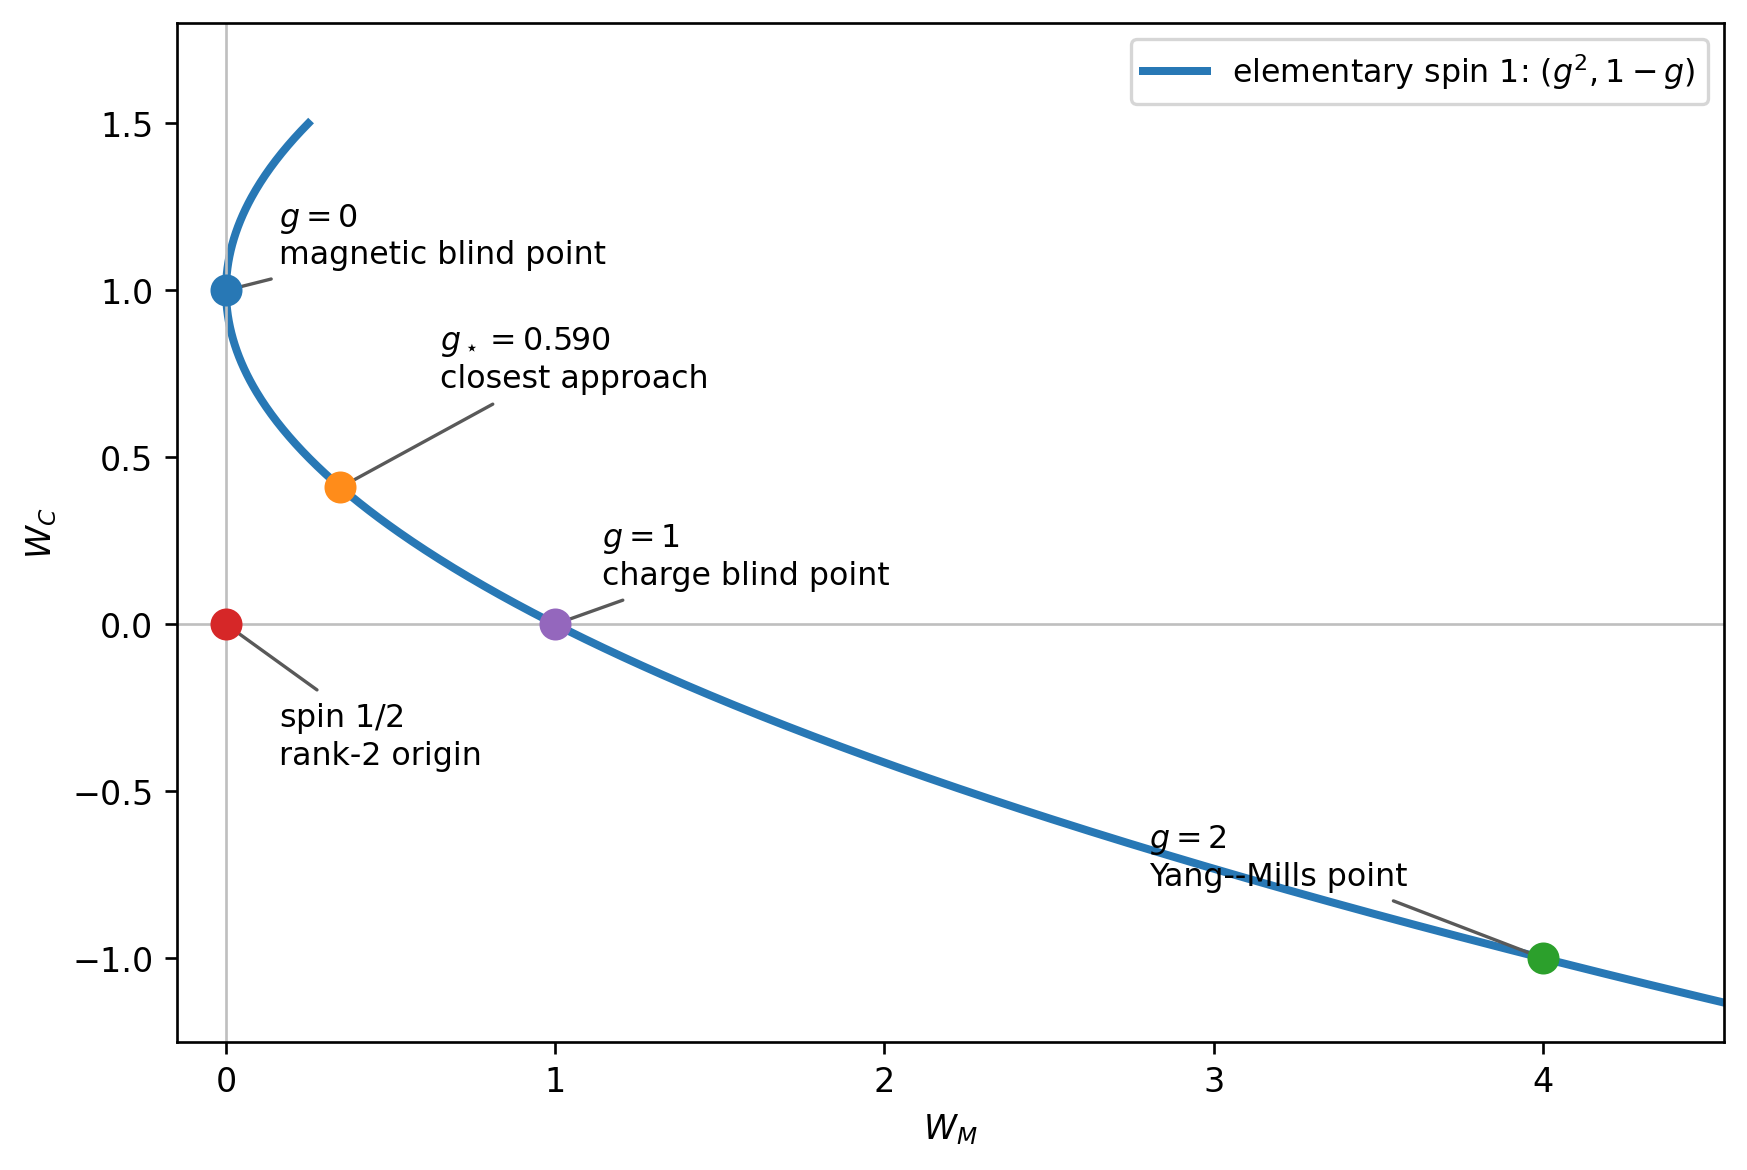
\includegraphics[width=0.72\textwidth]{figures/figure1a.png}\\[-0.5ex]
\textbf{(a)}\\[0.8ex]
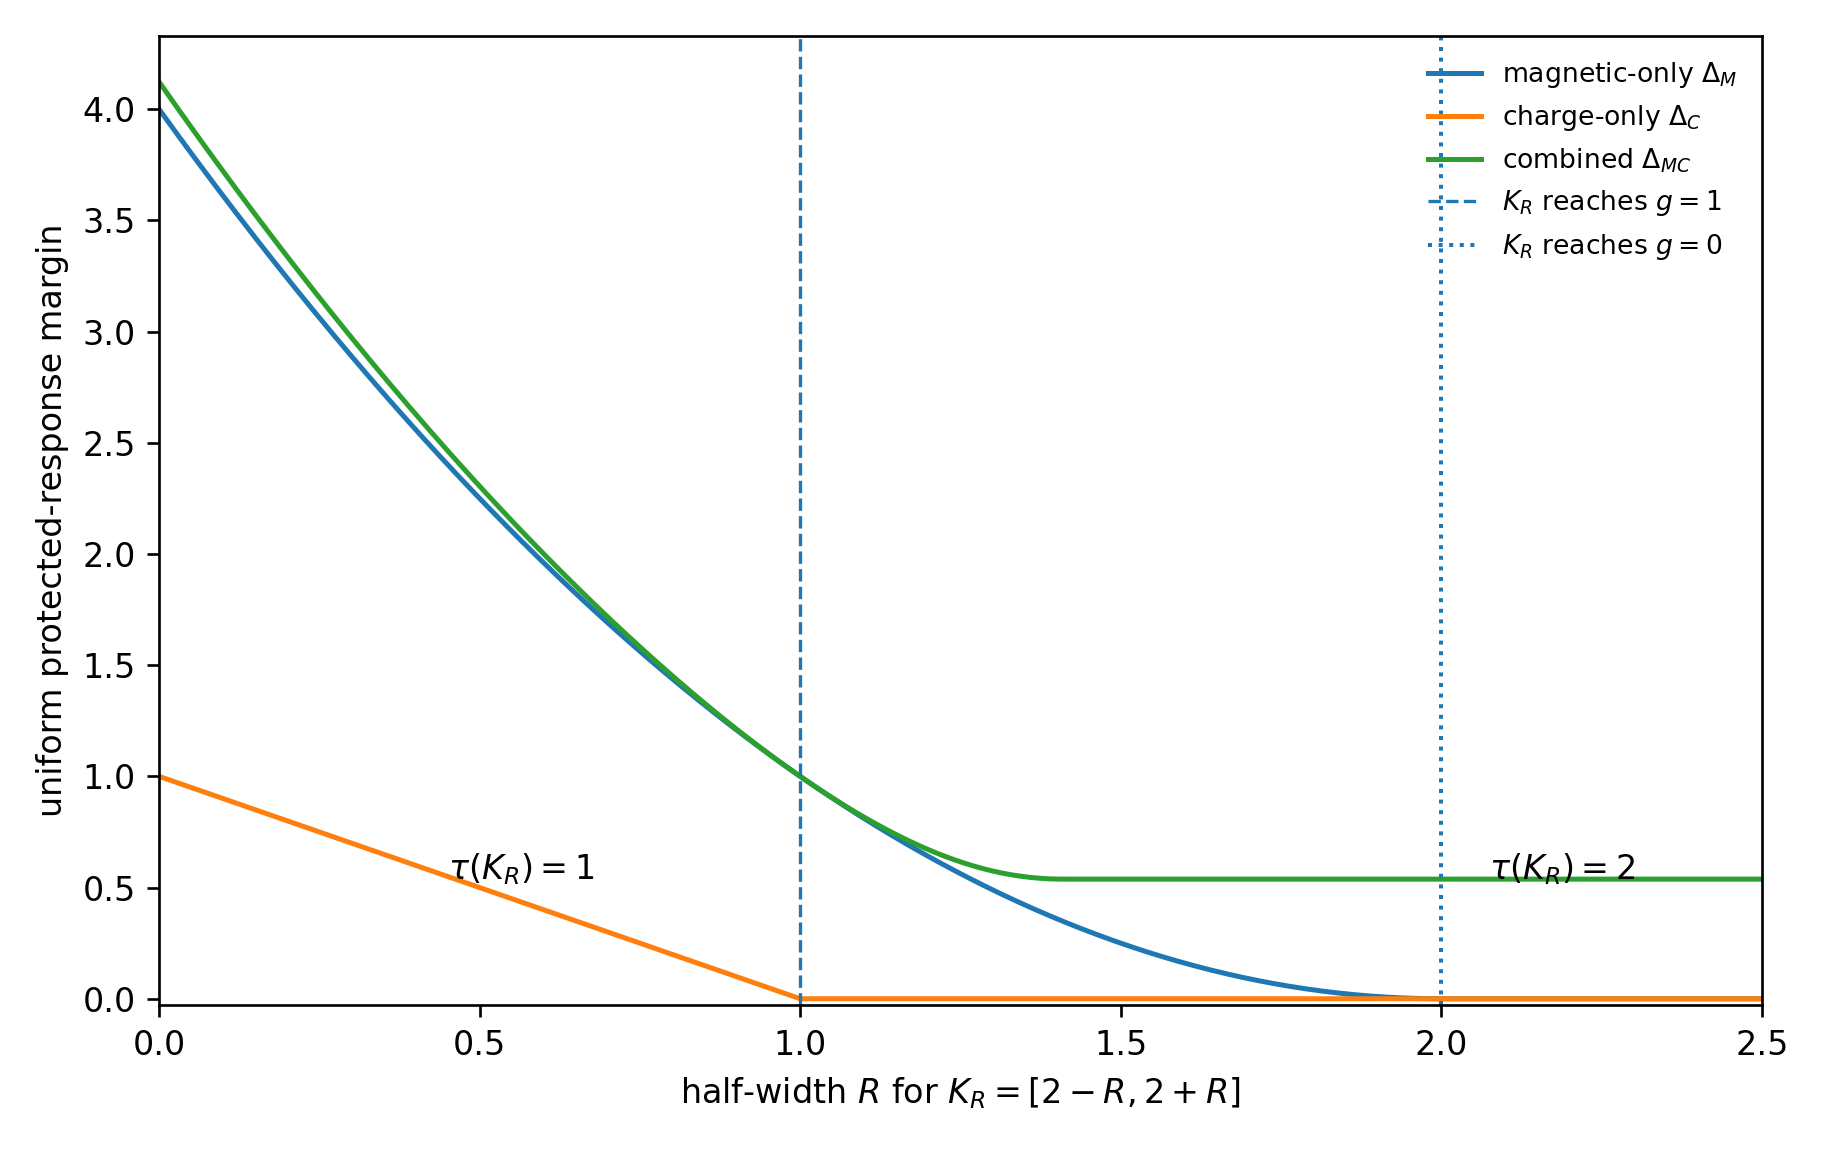
\includegraphics[width=0.72\textwidth]{figures/figure1b.png}\\[-0.5ex]
\textbf{(b)}
\alttext{Two-panel figure. Panel (a) plots the elementary spin-1 protected response curve with the spin-1/2 origin, the magnetic blind point at g=0, the charge blind point at g=1, the closest approach near g=0.590, and the Yang--Mills point g=2 marked. Panel (b) plots magnetic-only, charge-only, and combined uniform protected-response margins versus the half-width R of the interval K_R=[2-R,2+R]. The charge-only margin reaches zero at R=1 and the magnetic-only margin at R=2, while the combined margin remains positive.}
\caption{Static protected geometry and nuisance sensitivity. (a) Spin $1/2$ is fixed at the rank-$2$ origin, while the $\delta=0$ spin-$1$ slice follows $\bm W_1(g,0)=(g^2,1-g)$. The two primitive channels have blind points at $g=0$ and $g=1$, but the curve never reaches the origin. The Yang--Mills normalization $g=2$ is shown for reference. (b) For $K_R=[2-R,2+R]$, the charge-only margin vanishes at $R=1$, whereas the magnetic margin vanishes only at $R=2$. The combined protected margin remains strictly positive.}
\label{fig:static-geometry}
\end{figure}

\begin{remark}
\textbf{Scope.}
Equation~\eqref{eq:tau-K} applies to the specified primitive protected sector and to the admitted nuisance class in $(g,\delta)$. A strong ultraviolet or phenomenological prior localized near $g_M=2$ gives $\tau_{\mathrm{obs,prot}}=1$. Broader classes that retain both single-channel blind points require two primitive responses. A single readout that already accesses both primitive responses also has physical resource support two. Other measurement architectures, including polarization counting, spectroscopy, additional current components, or larger observable families, can provide different routes to spin identification.
\end{remark}

\section{Finite detector bandwidth and covariance-whitened robustness}
\label{sec:bandwidth}
% ============================================================

The static protected-sector criterion concerns the low-transfer limit. A finite detector samples a neighborhood of $Q^2=0$, and the correct robustness question is therefore uniform over an allowed smoothness class of form factors. Define
\begin{equation}
x=\frac{Q^2}{m^2}
\end{equation}
and use the reference-slice static constraints
\begin{equation}
G_1(0)=1,\qquad G_M(0)=g,\qquad G_Q(0)=1-g.
\end{equation}
The robustness extension replaces the final anchor by $G_Q(0)=1+\delta-g$ with $|\delta|\le\Delta$. We impose dimensionless Lipschitz bounds for every pair $x,y\ge0$,
\begin{equation}
|G_i(x)-G_i(y)|\le L_i|x-y|,
\qquad i\in\{1,M,Q\}.
\label{eq:lipschitz}
\end{equation}
For differentiable profiles this is equivalent to $|G_i'(x)|\le L_i$. For the piecewise-linear profiles below, the derivative bound holds almost everywhere and the definition includes their breakpoints.
In this conditional elastic model we take the spacelike form factors to be real valued, as used in the positive-effect decomposition above. The finite-bandwidth analysis uses a common bound $L_1=L_M=L_Q=L$. The original $99$-point classification is the $\delta=0$ slice. We report the compact prior $K=[1,3]$ and the broader stress-test domain $g\in[-4,4]$, which contains both blind points and the Standard Model $W$ point. The broad interval is chosen to stress-test the resource criterion across both single-channel blind points. The compact interval represents a theory-motivated neighborhood of $g_M=2$ and illustrates the nonblind regime.

The primary class is stated in the covariant vertex variables $(G_1,G_M,G_Q)$ because $G_1$ appears directly in Eq.~\eqref{eq:spin1-current} and in the regular off-shell completion that defines the elementary-field class. A transfer-dependent change of form-factor coordinates changes a common numerical Lipschitz constant. The coordinate choice is therefore part of the physical model. Using $G_1=G_C-xG_Q/6$, the same charge response can be written
\begin{equation}
\overline W_C=\int\dd\nu_C(x)\,
G_Q(x)\left[G_C(x)+\frac{x}{12}G_Q(x)\right].
\label{eq:finite-C-Sachs}
\end{equation}
We therefore repeat the sufficient whole-class test with the same $L$ imposed on $(G_C,G_M,G_Q)$. For the same pointwise box and $x\ge0$, $ab+xb^2/12\le ab+xb^2/4$, so the Sachs envelope cannot certify more points by construction. Only one of the $99$ outcomes changes. The covariant and Sachs tests certify $63$ and $62$ points, respectively. The Sachs sufficient test loses the cell $(\sigma_k/m,L)=(0.30,2)$, whose envelopes are $+0.008404$ and $-0.005405$. At the reference point the corresponding unit-covariance lower bounds are $0.403483$ and $0.402935$. The explicit overlap witness at $(0.15,8)$ also satisfies $\max|G_C'|\simeq7.791093<8$ and $\max|G_Q'|\simeq7.733996<8$. This witness belongs to both coordinate conventions. The remaining overlap labels refer to the covariant class.

We use the Lipschitz class as a deliberately broad stress test. At the largest $L$, it permits profiles that need not decrease across the sampled interval. A dispersive class would require additional quantitative input such as singularity locations and coefficient or spectral-norm bounds. Such information can reduce the admitted nuisance set and may shrink the overlap region. We leave that physically stronger class for future work.

For scale intuition, consider the unit-normalized dipole profile
\begin{equation}
\widehat G(Q^2)=\left(1+\frac{Q^2}{\Lambda^2}\right)^{-2}.
\end{equation}
Its origin slope in the dimensionless variable $x$ is
\begin{equation}
\left|\frac{\dd\widehat G}{\dd x}(0)\right|
=2\frac{m^2}{\Lambda^2},
\qquad
\frac{\Lambda}{m}=\sqrt{\frac{2}{L}}
\label{eq:dipole-proxy}
\end{equation}
when the slope bound is saturated. Thus $L=2$ corresponds to the proxy scale $\Lambda=m$, while $L=24$ corresponds to $\Lambda\simeq0.289m$. Equation~\eqref{eq:dipole-proxy} provides local scale intuition. For $G_i(Q^2)=G_i(0)\widehat G(Q^2)$ the absolute origin slope also contains $|G_i(0)|$. The common Lipschitz bound therefore leaves the dipole shape and structural scale free. The overlap boundary depends jointly on detector bandwidth and allowed softness. Explicit overlaps remain possible at $L=2$ for the broadest tested kernels.

Before introducing detector smearing, we state a stability result for the local, amplitude-calibrated protected coordinates (not yet for the bilinear finite-width charge effect). Let
\begin{equation}
\bm W_1(g,Q^2)=
\left(
|G_M(g,Q^2)|^2,\,
G_Q(g,Q^2)
\right),
\end{equation}
and let $\|\bm x\|_A=\sqrt{\bm x^{\mathsf T}A\bm x}$ for a fixed positive-definite matrix $A$.

\begin{proposition}
\textbf{Finite-transfer stability.}
\phantomsection\label{prop:finite-transfer}
Let $K\subset\mathbb R$ be compact and suppose $\bm W_1(g,Q^2)$ is jointly continuous on
$K\times[0,Q_{\max}^2]$. If
\begin{equation}
d_0=
\min_{g\in K}
\|\bm W_1(g,0)\|_A
>0,
\end{equation}
and for some $Q_\ast^2>0$
\begin{equation}
\sup_{g\in K}
\|\bm W_1(g,Q^2)-\bm W_1(g,0)\|_A
<d_0
\label{eq:finite-transfer-condition}
\end{equation}
for all $0\le Q^2\le Q_\ast^2$, then
\begin{equation}
\min_{g\in K}\|\bm W_1(g,Q^2)\|_A>0
\end{equation}
throughout that transfer interval. Hence the spin-$1$ protected response remains separated from the spin-$1/2$ origin.
\end{proposition}
\begin{proof}
For every $g\in K$, the reverse triangle inequality gives
\begin{align}
\|\bm W_1(g,Q^2)\|_A
&\ge
\|\bm W_1(g,0)\|_A
\nonumber\\
&\quad-
\|\bm W_1(g,Q^2)-\bm W_1(g,0)\|_A
\nonumber\\
&>
d_0-d_0=0.
\end{align}
Taking the minimum over the compact nuisance domain preserves strict positivity.
\end{proof}

Equation~\eqref{eq:finite-transfer-condition} is representation- and metric-aware and applies without choosing a particular form-factor ansatz. The explicit Lipschitz bounds below separately provide a constructive sufficient condition for the bilinear finite-width detector effect. The present local-coordinate statement alone does not imply the finite-width result.

With the explicit normalized measures in Eqs.~\eqref{eq:nuM-explicit} and \eqref{eq:nuC-explicit}, the finite-width rank-$2$ fingerprint is
\begin{align}
\overline W_M
&=\int \dd\nu_M(x)\,G_M^2(x),
\label{eq:finite-M}\\
\overline W_C
&=\int \dd\nu_C(x)
\left[G_1(x)G_Q(x)+\frac{x}{4}G_Q^2(x)\right].
\label{eq:finite-C}
\end{align}
In the zero-width limit, $(\overline W_M,\overline W_C)\rightarrow(g^2,1+\delta-g)$, with $\delta=0$ on the reference slice.

The Supplementary Material gives a componentwise moment bound for comparison. The nonnegative magnetic response also supplies a direct bound for the compact prior and the reduction used in the broad-class certificate.
\paragraph{Finite bandwidth under a nonblind magnetic prior.}
The magnetic channel can be analyzed independently of the charge form factor. Excluding its blind point gives a result for the complete anchored Lipschitz class at all finite bandwidths.

\begin{proposition}
\textbf{All-finite-bandwidth magnetic separation.}
\phantomsection\label{prop:magnetic-all-width}
Let the admitted magnetic-moment domain $K$ satisfy $g_0=\inf_{g\in K}|g|>0$. For every finite $L\ge0$ and every Gaussian width $0<\sigma_k/m<\infty$, the calibrated magnetic response satisfies
\begin{equation}
\boxed{\overline W_M\ge M_L(g_0):=\int\dd\nu_M(x)\,[\max(g_0-Lx,0)]^2>0.}
\label{eq:compact-magnetic-margin}
\end{equation}
Consequently, the magnetic channel alone separates the spin-$1$ and spin-$1/2$ protected model sets for the entire admitted Lipschitz class. This statement is independent of $g_Q$ and therefore holds for arbitrary $\delta$.
\end{proposition}
\begin{proof}
The Lipschitz condition and $|G_M(0)|\ge g_0$ give $|G_M(x)|\ge\max(g_0-Lx,0)$ for every $x\ge0$. Squaring and integrating against the normalized positive measure $\nu_M$ proves the lower bound. For $L>0$ the integrand is positive on $0\le x<g_0/L$. For $L=0$ it is the positive constant $g_0^2$. Every finite-width Gaussian magnetic measure assigns positive mass to a neighborhood of $x=0$, so the integral is strictly positive.
\end{proof}

For $K=[1,3]$ we have $g_0=1$. For $K_R=[2-R,2+R]$ with $0\le R<2$, we have $g_0=2-R$. The $99$-point grid evaluates the size of the analytic margin, not the range of validity of Proposition~\ref{prop:magnetic-all-width}. At $L=2$ and $K=[1,3]$, the magnetic margins are $0.888252$ for $\sigma_k/m=0.10$ and $0.160533$ for $\sigma_k/m=0.50$. The smallest grid value is $0.005136$ at $(0.50,24)$. The full numerical table and quadrature script are publicly available in the repository identified in the Data availability statement.

\begin{theorem}
\textbf{Whole-class finite-bandwidth certificate on the $\delta=0$ slice.}
\phantomsection\label{prop:positivity-envelope}
Assume the form factors are continuous and $0\in\overline{\operatorname{supp}\nu_M}$. A protected-origin overlap,
\begin{equation}
(\overline W_M,\overline W_C)=(0,0),
\end{equation}
requires
\begin{equation}
g=0,
\qquad
G_M(x)\equiv0
\label{eq:magnetic-zero-reduction}
\end{equation}
on the detector support. For the common anchored Lipschitz bound $L$, define
\begin{equation}
h_L(x)=
\min_{a,b\in[1-Lx,1+Lx]}
\left[ab+\frac{x}{4}b^2\right]
\label{eq:charge-envelope}
\end{equation}
and
\begin{equation}
B_C(\sigma_k/m,L)=\int\dd\nu_C(x)\,h_L(x).
\label{eq:BC}
\end{equation}
Then every admissible profile satisfying $\overline W_M=0$ obeys
\begin{equation}
\overline W_C\ge B_C(\sigma_k/m,L).
\end{equation}
Consequently, $B_C>0$ excludes a joint protected-origin overlap for the complete anchored Lipschitz class with $g\in[-4,4]$.
\end{theorem}
\begin{proof}
Under the stated hypothesis $\overline W_M=0$, the integrand in Eq.~\eqref{eq:finite-M} is nonnegative. Its integral can vanish only if $G_M=0$ almost everywhere with respect to the positive measure. Continuity extends this equality to $\overline{\operatorname{supp}\nu_M}$. Because that closed support contains the anchor, $g=G_M(0)=0$. The static constraint then gives $G_1(0)=G_Q(0)=1$. At each transfer $x$, the Lipschitz condition implies $G_1(x),G_Q(x)\in[1-Lx,1+Lx]$. Pointwise minimization of the charge integrand gives Eq.~\eqref{eq:charge-envelope}. Integration against the positive normalized measure gives Eq.~\eqref{eq:BC}.
\end{proof}

\begin{corollary}
\textbf{Uniform robustness to the moment-relation deformation.}
\phantomsection\label{cor:delta-robustness}
Let $|\delta|\le\Delta$. After the magnetic reduction in Eq.~\eqref{eq:magnetic-zero-reduction}, define
\begin{equation}
h_{L,\Delta}(x)=
\min_{\substack{a\in[1-Lx,1+Lx]\\
b\in[1-\Delta-Lx,1+\Delta+Lx]}}
\left[ab+\frac{x}{4}b^2\right]
\label{eq:charge-envelope-delta}
\end{equation}
and
\begin{equation}
B_C(\sigma_k/m,L,\Delta)=\int\dd\nu_C(x)\,h_{L,\Delta}(x).
\label{eq:BC-delta}
\end{equation}
Every admissible profile in the enlarged class satisfies $\overline W_C\ge B_C(\sigma_k/m,L,\Delta)$ whenever $\overline W_M=0$. Hence $B_C>0$ excludes a protected-origin overlap uniformly over $|\delta|\le\Delta$.
\end{corollary}
\begin{proof}
The magnetic reduction again gives $g=0$. The anchor of $G_Q$ is then $1+\delta$, so the union of all allowed pointwise values for $|\delta|\le\Delta$ is contained in $[1-\Delta-Lx,1+\Delta+Lx]$. The same pointwise minimization and integration used in Theorem~\ref{prop:positivity-envelope} gives the result.
\end{proof}

At $\Delta=0$ the corollary reduces to Theorem~\ref{prop:positivity-envelope}. On the same $99$-point grid, the number of whole-class certificates is $63$ at $\Delta=0$, $61$ at $\Delta=0.10$, $59$ at $\Delta=0.25$, and $55$ at $\Delta=0.50$. The $33$ existing overlap witnesses remain admissible because the enlarged classes contain the $\delta=0$ slice. At the reference point $(\sigma_k/m,L)=(0.10,2)$, the uniform charge lower bound is $0.735957$ for $\Delta=0.10$. The full robustness table is reported in the Supplementary Material and reproduced by the public audit script.

For numerical evaluation, the minimum in Eq.~\eqref{eq:charge-envelope} is elementary. At fixed $b$ the expression is linear in $a$, so $a$ lies at one of the two interval endpoints. For either endpoint the remaining function of $b$ is a convex quadratic and its constrained minimum is obtained by clipping $b=-2a/x$ to the same interval. This evaluates the envelope without an inner stochastic optimizer.

The pointwise construction relaxes the anchored Lipschitz minimization by selecting the minimizing pair $(a,b)$ independently at each $x$. The resulting analytic lower bound is valid for the complete anchored Lipschitz class and can be conservative. A value $B_C\le0$ leaves the point undecided and can coexist with a positive minimum in the finite piecewise-linear audit, as occurs at the three unresolved points.

On the $\delta=0$ slice, the same pointwise construction also yields a quantitative whole-class distance. For each anchor $g$, define
\begin{align}
M_L(g)&=\int\dd\nu_M(x)\,[\max(|g|-Lx,0)]^2,
\label{eq:magnetic-floor}\\
C_L^\pm(g)&=\int\dd\nu_C(x)\,
\underset{\substack{a\in[1-Lx,1+Lx]\\
b\in[1-g-Lx,1-g+Lx]}}{\operatorname{ext}_{\pm}}
\left(ab+\frac{x}{4}b^2\right),
\label{eq:charge-range}
\end{align}
where $\operatorname{ext}_{-}$ and $\operatorname{ext}_{+}$ denote the pointwise minimum and maximum.

\begin{proposition}
\textbf{Whole-class distance enclosure.}
\phantomsection\label{prop:distance-enclosure}
Every admissible fingerprint with anchor $g$ lies in
\begin{equation}
\mathcal R_L(g)=[M_L(g),\infty)\times[C_L^-(g),C_L^+(g)].
\end{equation}
Consequently, for any positive-definite precision matrix $A$ and compact anchor domain $K$, the true covariance-whitened class distance from the spin-$1/2$ origin obeys
\begin{equation}
\inf_{\bm W\in\mathcal W_1}\|\bm W\|_A
\ge D_L(A)\equiv
\min_{g\in K}\min_{\bm u\in\mathcal R_L(g)}\|\bm u\|_A.
\label{eq:whole-class-distance}
\end{equation}
\end{proposition}
\begin{proof}
The anchored Lipschitz condition gives $|G_M(x)|\ge\max(|g|-Lx,0)$, proving the first coordinate bound after squaring and integrating.  The charge integrand lies between its exact extrema over the displayed rectangle at every $x$, proving the second coordinate interval after integration.  Thus the admissible model set is contained in $\bigcup_{g\in K}\mathcal R_L(g)$, and minimizing a norm over this larger set can only decrease the true class distance.
\end{proof}

For fixed $g$, the inner problem in Eq.~\eqref{eq:whole-class-distance} is a two-variable convex quadratic minimization over a half-strip and is evaluated from its boundary stationary points.  The remaining scalar minimization over $g\in[-4,4]$ is deterministic.  Like $B_C$, the enclosure is conservative because its pointwise extrema need not form one common Lipschitz profile.

At $(\sigma_k/m,L)=(0.10,2)$ with unit covariance on the $\delta=0$ slice, this lower enclosure gives $0.4034833471$. An explicit admissible family,
\begin{equation}
\begin{aligned}
G_M&=\operatorname{sgn}(g)\max(|g|-Lx,0),\\
G_1&=1-Lx,\qquad G_Q=1-g-Lx,
\end{aligned}
\label{eq:explicit-distance-upper-profile}
\end{equation}
minimized at $g=0.5734946$, gives $0.4034946602$. Hence the true class distance obeys the tight bracket
\begin{equation}
\boxed{0.403483\le d_{\rm class}\le0.403495.}
\label{eq:reference-distance-bracket}
\end{equation}
The decimal values are numerical evaluations of the analytic enclosure and are checked by grid and Gaussian-tail convergence. Formal interval arithmetic is not used. The lower-bound calculation is also evaluated at every point of the $99$-point grid. Figure~\ref{fig:bandwidth-status}(b) displays the resulting quantitative map. The full machine-readable table is available in the public repository, and the quadrature and Gaussian-tail convergence checks are documented in the Supplementary Material.

In parallel, piecewise-linear form factors satisfying the same slope bounds are optimized adversarially to search for an explicit model whose finite-width fingerprint reaches the spin-$1/2$ origin. A successful construction proves an overlap within the discretized Lipschitz class. An unsuccessful search leaves separation undecided. We therefore use three labels, \emph{guaranteed separation}, \emph{explicit overlap found}, and \emph{unresolved}. This keeps constructive evidence separate from whole-class certification.

For finite-noise data, let $\Sigma$ be the covariance matrix of the calibrated fingerprint estimator. The relevant distance is
\begin{equation}
\Delta_\Sigma(\bm W,\bm W')=
\sqrt{(\bm W-\bm W')^{\mathsf T}\Sigma^{-1}(\bm W-\bm W')}.
\label{eq:mahalanobis}
\end{equation}
Write
\begin{equation}
\Sigma=\varepsilon^2\Sigma_{\mathrm{shape}},
\end{equation}
so $\Sigma_{\mathrm{shape}}$ fixes relative channel precision and correlation, while $\varepsilon$ sets a reference estimator-uncertainty scale. In the Supplementary Material convention $\Sigma_{\mathrm{shape}}=\bigl(\begin{smallmatrix}1&\rho r_\Sigma\\ \rho r_\Sigma&r_\Sigma^2\end{smallmatrix}\bigr)$, $\varepsilon=\sigma(W_M)$ and $r_\Sigma\varepsilon=\sigma(W_C)$. The parameter $\varepsilon$ is a magnetic-coordinate reference scale and becomes a common standard deviation only when $r_\Sigma=1$.

The componentwise moment bound certifies 46 of the 99 bandwidth--smoothness points. Theorem~\ref{prop:positivity-envelope} certifies 17 further points for the complete Lipschitz class. A simple two-kink continuous family produces explicit overlap paths in all 33 overlap cells; the $(\sigma_k/m,L)=(0.15,8)$ example illustrates the corresponding high-resolution root. For the $\delta=0$ reference slice, the final classification is
\begin{equation}
\boxed{63\ \text{certified},\qquad
33\ \text{explicit overlaps},\qquad
3\ \text{unresolved}.}
\label{eq:status-63-33-3}
\end{equation}
A deterministic two-kink family provides a direct constructive witness for every one of the 33 overlap cells, without relying on the optimizer's convergence:
\begin{align}
X_\sigma&=2\!\left[\sqrt{1+(9\sigma_k/m)^2}-1\right],
&h_\sigma&=X_\sigma/32,\notag\\
G_M^{(t)}(x)&=0,\qquad
G_Q^{(t)}(x)=1-tL\min(x,X_\sigma),\notag\\
G_1^{(t)}(x)&=1+tL\!\left[\min(x,X_\sigma)-2\min(x,h_\sigma)\right],
\qquad 0\le t\le1.
\label{eq:two-kink-witness}
\end{align}
All profiles are anchored correctly and have slopes of magnitude at most $L$. At $t=0$, the charge response is positive; knot-split quadrature gives $\overline W_C(1)<0$ for all 33 overlap cells, the least negative value being approximately $-0.0474608$ at $(0.15,8)$. Continuity in $t$ proves an exact protected-origin overlap in each such cell. The full set of 33 signed values and roots is provided with the reproducibility audit; the numerical sign checks are not formal interval-arithmetic certificates.

The three points not classified by either whole-class positivity or the two-kink witness are $(0.08,24)$, $(0.10,16)$, and $(0.50,1)$. Their newly evaluated eight-segment global QCQP minima are $0.201665$, $0.168785$, and $0.105516$, respectively. These finite-basis positive minima do not certify the complete Lipschitz class, and the three points remain unresolved. The old 32-segment multistart values obtained with the filtered charge measure are not reused. An explicit overlap occurs at $L(\sigma_k/m)^2=0.18$, while whole-class certificates persist at some tested points up to $0.25$. The low-transfer product remains a useful organizing variable, but the relativistic detector measure prevents exact one-parameter scaling.

For the $(0.15,8)$ overlap, the family in Eq.~\eqref{eq:two-kink-witness} is the same as a 32-segment profile with its first $G_1$ slope negative, its remaining $G_1$ slopes positive, and every $G_Q$ slope negative. It gives
\begin{equation}
\overline W_C(0)=1.0263573066,
\qquad
\overline W_C(1)\simeq-0.0474607720,
\end{equation}
when its slopes are scaled continuously by $t\in[0,1]$. The verified root is
\begin{equation}
t_\star\simeq0.9667494646,
\qquad
|\overline W_C(t_\star)|\sim10^{-15}\quad\text{(unrounded numerical root)},
\end{equation}
and its maximum absolute slope is $7.7339957<8$. The displayed numerical root uses continuous quadrature split at the segment knots; the exact existence assertion follows instead from the positive-to-negative endpoint sign change and the intermediate-value theorem. Together with $\overline W_M=0$, this is an explicit protected-origin overlap in the full admissible class.

We also audit the 21 points inconclusive under the componentwise bound in an eight-segment basis. After Eq.~\eqref{eq:magnetic-zero-reduction}, the charge response is a box-constrained QCQP that is linear in the eight $G_1$ slopes. Enumerating all $2^8$ vertices and solving the remaining convex box QP in the eight $G_Q$ slopes gives a positive global finite-basis minimum at every one of the 21 points, with numerical KKT residuals checked at the reported minima. A separate degree-$2$ SOS calculation supplies explicit numerically feasible positive lower bounds for at least 12 of the 21 unreduced bilinear QCQPs; negative relaxation bounds remain inconclusive. The finite-basis minima and SOS identities audit the numerical procedure. Whole-class certification uses the analytic envelope in Theorem~\ref{prop:positivity-envelope}.

\begin{figure}[t]
\centering
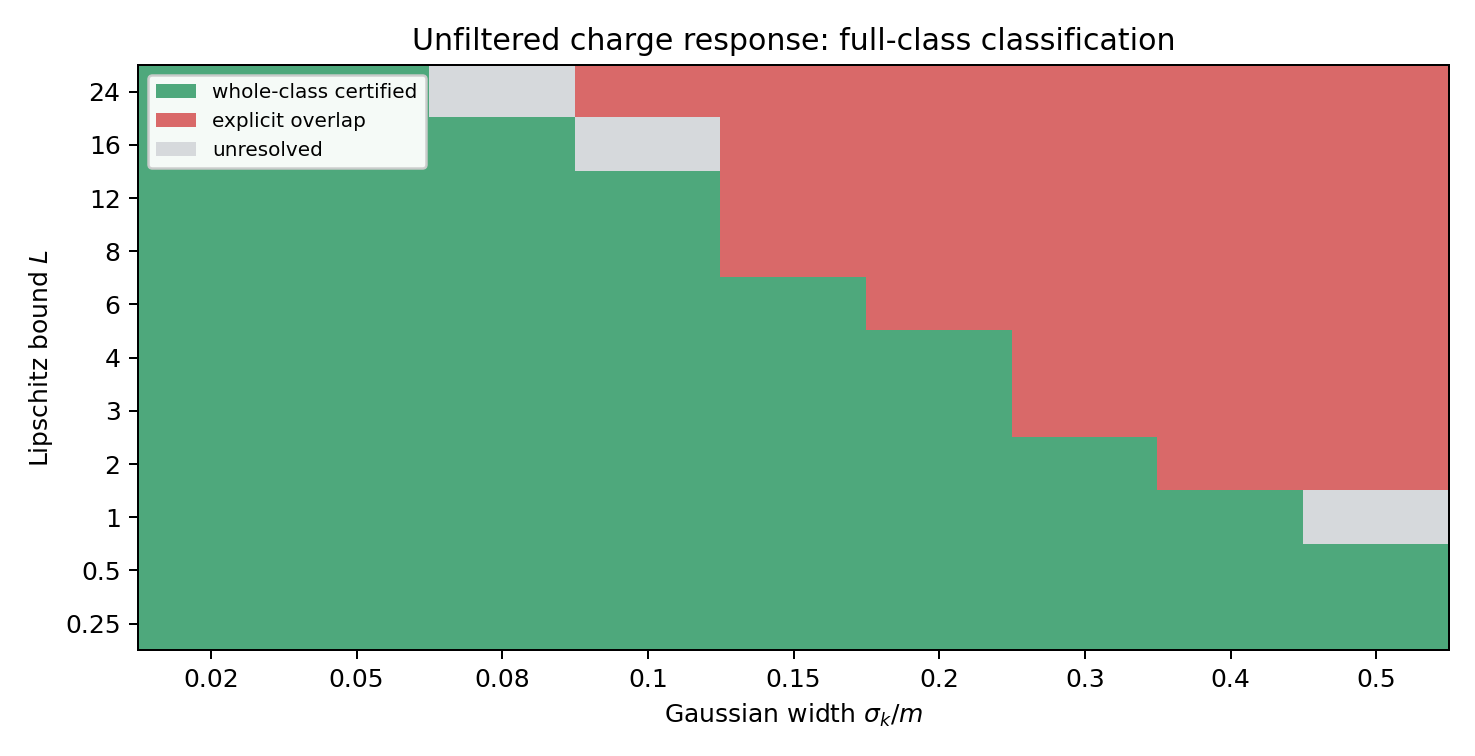
\includegraphics[width=0.72\textwidth]{figures/figure2a.png}\\[-0.5ex]
\textbf{(a)}\\[0.8ex]
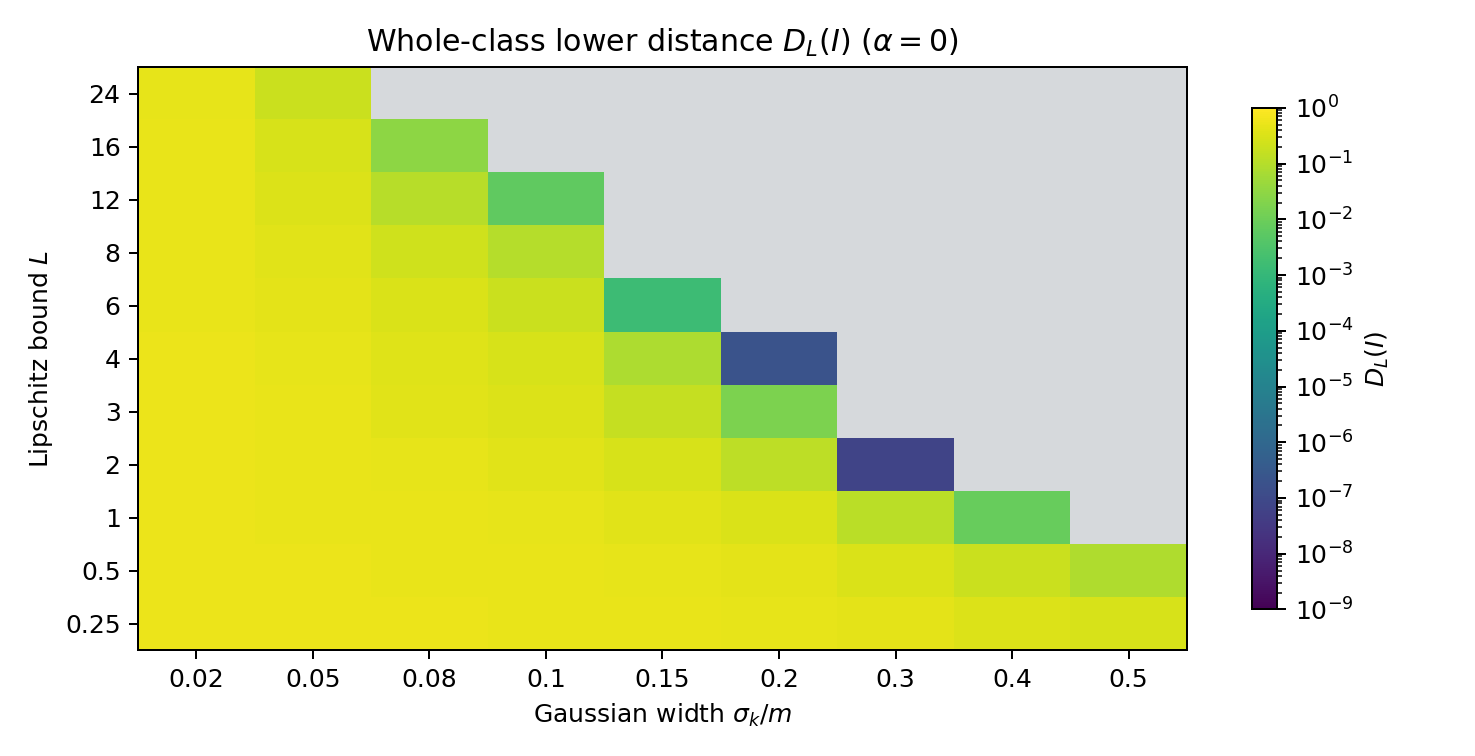
\includegraphics[width=0.72\textwidth]{figures/figure2b.png}\\[-0.5ex]
\textbf{(b)}
\alttext{Two-panel bandwidth--smoothness grid over 99 tested points. Panel (a) classifies points as whole-class certified, explicit overlap, or unresolved. The unresolved points are (sigma_k/m,L)=(0.08,24), (0.10,16), and (0.50,1). Panel (b) shows the whole-class unit-covariance lower bound D_L(I) on the same grid on a logarithmic scale. Cells with zero lower enclosure are inconclusive.}
\caption{Finite-bandwidth protected-sector geometry on the $\delta=0$ reference slice after positivity reduction. (a)~Green points have a whole-Lipschitz certificate, red points contain an explicit admissible spin-$1$ profile reaching the spin-$1/2$ protected origin, and the three gray points remain unresolved. Magnetic positivity places every red overlap at the broad-class blind value $g_M=0$. The natural point $g_M=2$ is outside this degeneracy. (b)~Whole-class unit-covariance lower bound $D_L(I)$ on the same $99$-point grid. The logarithmic color scale quantifies the certified margin. Gray cells have zero half-strip lower bound and are classified separately by the constructive overlap search.}
\label{fig:bandwidth-status}
\end{figure}

\FloatBarrier

% ============================================================
\section{Estimator-space interpretation and consistency tests}
\label{sec:statistical}
% ============================================================

The finite-bandwidth calculation determines physical model-space separation. Statistical performance also depends on the precision of the two fingerprint coordinates. The scale $\varepsilon$ below is an estimator-uncertainty parameter. Converting $\varepsilon$ to an event count requires a concrete likelihood or estimating equation and its per-event covariance, or equivalently the corresponding Fisher information. We therefore report the result directly in estimator space and model the extracted fingerprint as
\begin{equation}
\widehat{\bm W}\sim
\mathcal N(\bm W,\varepsilon^2\Sigma_{\mathrm{shape}})
\label{eq:estimator-model}
\end{equation}
and calibrate a profile-distance test to a $5\%$ false-positive rate under spin $1/2$.

At the reference point $\sigma_k/m=0.10$, $L=2$, and $\Sigma_{\mathrm{shape}}=I$, the validation uses 8000 Monte Carlo estimator draws per hypothesis. The quoted powers average over a specified inference cloud. We draw $g$ uniformly on $[-4,4]$ and the 24 slopes of the three eight-segment form factors independently and uniformly on $[-2,2]$. The cloud-averaged spin-$1$ power is $0.881$ at $\varepsilon=0.50$, $0.961$ at $\varepsilon=0.30$, $0.992$ at $\varepsilon=0.20$, and $0.999$ at $\varepsilon=0.15$. The corresponding ROC areas are $0.969$, $0.992$, $0.998$, and $0.9997$. These values are nuisance averaged. For the explicit near-boundary profile at $g=0.573495$ that supplies the upper endpoint of Eq.~\eqref{eq:reference-distance-bracket}, the powers at the same four uncertainty scales are $0.166$, $0.357$, $0.629$, and $0.824$. The two sets of values quantify estimator precision for the stated nuisance sampling and boundary profile.

At the same reference point, Proposition~\ref{prop:distance-enclosure} and the explicit profile in Eq.~\eqref{eq:explicit-distance-upper-profile} bracket the equal-error class distance between $0.403483$ and $0.403495$. The whole-class lower bound falls to $0.150643$ if the charge-coordinate standard deviation is four times the magnetic-coordinate standard deviation. These values follow from the explicit measures and deterministic scalar minimizations. The full $99$-point distance map and the grid and Gaussian-tail convergence tests are tabulated in the Supplementary Material. The finite-noise geometry therefore depends materially on the covariance shape.

A detector ablation checks the broad-class resource criterion at finite bandwidth. At $\sigma_k/m=0.10$ and $L=2$, adversarial optimization drives the magnetic-only gap below $10^{-21}$ and the charge-only gap below $5\times10^{-9}$, while the two-channel unit-covariance distance satisfies the independently derived bracket in Eq.~\eqref{eq:reference-distance-bracket}. Thus each primitive channel can still be tuned away separately, while their combination remains separated at the reference point.

The expanded nuisance class makes the failure mode explicit. If it admits $g=0$ and $\delta=-1$, then $g_Q=0$ and the protected spin-$1$ fingerprint reaches the spin-$1/2$ origin exactly. The rank-$2$ representation difference alone is therefore insufficient for this certificate. Equation~\eqref{eq:tau-K} identifies the precise blind locus in the enlarged moment-relation class.

Detailed estimator-space power curves, covariance-shape scans, and the complete numerical protocol are reported in the Supplementary Material \cite{SupplementalMaterial}.

% ============================================================
\section{Extension to other spin pairs}
\label{sec:computational}
% ============================================================

The architecture-aware criterion has a direct geometric extension beyond the spin-$1/2$--spin-$1$ example. Order the pair as $s<s'$, and let $\Pi_{>2s}$ project onto internal rotational ranks unavailable to spin $s$. For a higher-spin nuisance domain $\Xi_{s'}$, define the protected model set
\begin{equation}
\mathcal V_{s'|s}
=\left\{\Pi_{>2s}\bm W_{s'}(\xi):\xi\in\Xi_{s'}\right\}
\subseteq\mathcal R_{\mathcal A}.
\label{eq:protected-variety}
\end{equation}
The lower-spin protected set is the origin. For each physical block $a\in\mathcal A$, define its blind locus
\begin{equation}
Z_a=\left\{\xi\in\Xi_{s'}:
\pi_a\Pi_{>2s}\bm W_{s'}(\xi)=0\right\}.
\label{eq:blind-locus}
\end{equation}
Then Eq.~\eqref{eq:general-threshold} becomes
\begin{equation}
\boxed{
\tau_{\mathcal A}(s,s')
=\min_{S\subseteq\mathcal A}
\left\{|S|:\bigcap_{a\in S}Z_a=\varnothing\right\}.}
\label{eq:higher-spin-threshold}
\end{equation}
This statement is abstract but exact. It reduces the resource problem to the existence of a common admissible nuisance point in the selected detector-block blind loci. The relevant higher-spin multipole constraints must be established independently for the physical model class under study.

For finite polynomial parametrizations, the resulting model-set intersection can be relaxed through moment and sum-of-squares methods \cite{Lasserre2001,Parrilo2003}. The degree-$2$ identity used in the finite-bandwidth audit is one directly checkable relaxation. Its explicit matrix form and verification residuals are given in the Supplementary Material. A positive certificate proves separation in the stated parametrization. A nonpositive relaxation remains inconclusive for the full function class.

% ============================================================
\section{Discussion}
\label{sec:discussion}

The central result is a nuisance-class-dependent detector-resource criterion for spin identification. Proposition~\ref{prop:magnetic-all-width} gives a whole-class magnetic margin at every finite Gaussian bandwidth and finite Lipschitz bound whenever the admitted domain stays away from $g_M=0$. A second primitive response becomes necessary for static uniform separation only after the admitted class includes both single-channel blind points. Finite-width exact overlaps in the broad class show that detector blindness can persist even when both calibrated responses are available. More observations reduce statistical error when the accessible responses differ. They cannot resolve an exact response degeneracy.

For charged spin-$1/2$ versus spin-$1$ particles, the protected rank-$2$ sector makes the distinction explicit. Spin $1/2$ cannot support this internal sector, while spin $1$ can. In the enlarged class $g_M+g_Q=1+\delta$, a joint protected blind point requires $(g,\delta)=(0,-1)$. The two primitive responses therefore remain statically separating for every compact deformation domain that excludes $\delta=-1$.

The architecture-aware threshold counts physical inputs. Although $W_M+W_C$ is one scalar and never vanishes on the elementary static spin-$1$ curve, obtaining it requires access to both primitive responses. If the higher-spin class admits independently variable magnetic and quadrupole moments, it can contain $g_M=g_Q=0$ and the protected certificate disappears. The elementarity hypothesis is therefore a substantive input to the comparison.

Finite bandwidth tests the robustness of this distinction. Magnetic positivity reduces every possible origin overlap to $g_M=0$ and removes the magnetic form factor on the detector support. Proposition~\ref{prop:magnetic-all-width} is unchanged by $\delta$. Corollary~\ref{cor:delta-robustness} gives a whole-class envelope uniform over $|\delta|\le\Delta$. On the reference grid, $61$ points remain certified at $\Delta=0.10$ and $55$ at $\Delta=0.50$. The $\delta=0$ slice contains the explicit continuous-class degeneracies and the three unresolved points reported above.

Restricted measurements, informational completeness, and observable reconstruction provide the inverse-problem setting \cite{MatthewsWehnerWinter2009,Finkelstein2004,BaldwinDeutschKalev2016,ArenhoevelFix2014,CaretteGlowackiLoveridge2023,DuEtAl2026}. Our contribution is a detector-resource criterion for the elementary current class together with finite-bandwidth certification over the complete anchored Lipschitz class. The broad nuisance class also yields constructive degeneracies, so the analysis identifies both the separating region and its failure modes. Finite-basis QCQP and SOS calculations use established optimization methods \cite{Lasserre2001,Parrilo2003} to audit the numerical boundary.

The protected-variety and blind-locus formulation extends the criterion to other spin pairs once their physical nuisance classes are specified. For adjacent spins, the first new internal rank is $\ell=2s+1$. Under Lorc\'e's additional pointlike light-cone-helicity prior, the corresponding natural multipole is fixed and nonzero \cite{Lorce2009NaturalMoments}. Applying the same geometric criterion to a broader EFT class requires the corresponding higher-spin consistency constraints.


\section{Conclusion}
\label{sec:conclusion}

We formulated charged-particle spin identification as a detector-restricted inverse problem in QFT. The architecture-aware criterion separates intrinsic representation content from the physical responses available to an experiment. Increasing statistics cannot remove an exact detector-response degeneracy. Spin identification then requires additional physical information or an independently justified restriction of the model class.

For charged spin-$1/2$ and spin-$1$ candidates, the rank-$2$ sector and the spin-$1$ moment constraints give complementary magnetic and charge-sensitive protected responses. Writing $g_M+g_Q=1+\delta$ makes the dependence on the theory-side current class explicit. Proposition~\ref{prop:magnetic-all-width} proves that any magnetic-moment class bounded away from $g_M=0$ has a positive magnetic-only margin at every finite Gaussian bandwidth and finite Lipschitz bound, independently of $\delta$. The interval $K=[1,3]$ supplies a concrete example.

On the Haberzettl slice $\delta=0$, the broad interval $g_M\in[-4,4]$ yields 63 whole-class certificates, 33 explicit overlaps, and three unresolved points. Every constructed origin overlap occurs at $g_M=0$. Enlarging the moment relation to $|\delta|\le0.10$ retains 61 whole-class certificates, and the reference finite-width lower bound remains positive. Static two-channel separation can fail only when the nuisance domain reaches $\delta=-1$. The higher-spin extension reduces the same resource question to intersections of detector-block blind loci once the relevant physical constraints are fixed.


\funding{This work was supported by the University of Zagreb Faculty of Organization and Informatics through the Institutional Research Projects funded under the National Recovery and Resilience Plan 2021--2026, under the project ``PiPi: Data Infrastructure and Augmented Intelligence for Sustainable Development.''}

\ack{ChatGPT and Codex (OpenAI, GPT-5-series models, accessed in 2026) were used for language editing, code debugging, and consistency checks. The author reviewed the resulting text and computational changes and takes full responsibility for the scientific content, analyses, and reported results.}

\data{The unfiltered-charge ($\alpha=0$) numerical code, processed data, and reproducibility checks are publicly available in the project repository at the fixed scientific snapshot~\cite{VlahekSpinRepo2026}. They include the 99-point whole-class classification, 33 signed two-kink witnesses, covariance and distance enclosures, QCQP/SOS numerical audits, estimator-space checks, and the $\delta$-robustness calculation. The older filtered-charge ($\alpha=2$) results are retained separately as development provenance and should not be used to reproduce the present tables.}

\suppdata{Supplementary material accompanies this article and contains the numerical protocols, nuisance-class robustness results, finite-basis audits, and estimator-space checks.}

\FloatBarrier
\section*{References}
\printbibliography[heading=none]

\end{document}
